\section{Análisis de los diez sitios más visitados de la actualidad.}
\label{capitulo3:sitios_visitados}
Luego de haber analizado las reglas de Steve Souders en la Sección \ref{capitulo3:reglas} y las herramientas que existen actualmente para medir la performance del lado cliente en la Sección \ref{capitulo3:herramientas}, se decidió analizar el estado actual de
los diez sitios más visitados a nivel mundial según el ranking propuesto
por Alexa \cite{alexa}. Se presenta a continuación la lista de sitios ordenadas en forma decreciente por cantidad de visitas:

\begin{enumerate}
	\item
	\textbf{\emph{Google.}} www.google.com
	\item
	\textbf{\emph{Facebook.}} www.facebook.com
	\item
	\textbf{\emph{Youtube.}} www.youtube.com
	\item
	\textbf{\emph{Yahoo}} www.yahoo.com
	\item
	\textbf{\emph{Baidu.}} www.baidu.com
	\item
	\textbf{\emph{Wikipedia.}} www.wikipedia.org
	\item
	\textbf{\emph{Live.(Microsoft)}} www.live.com
	\item
	\textbf{\emph{QQ.}} www.qq.com
	\item
	\textbf{\emph{Twitter.}} www.twitter.com
	\item
	\textbf{\emph{Amazon.}} www.amazon.com
\end{enumerate}

Dado que las reglas escritas por Souders no son demasiado actuales, parece razonable realizar un nuevo análisis acerca de cómo los sitios más concurridos mundialmente se
comportan respecto a la performance. En las siguientes subsecciones se detallará el estado actual de los sitios viendo entre otras cosas puntos de falla comunes y datos
particularmente relevantes. Las herramientas que se utilizaron para recabar datos de performance son \emph{Page Speed}\cite{page_speed} y \emph{Web Page
Test}\cite{web_page_test}.

\emph{Page Speed} es una herramienta \emph{open source} desarrollada por Google la cual se instala como complemento al navegador (disponible tanto para chrome como firefox).
La misma realiza varias pruebas sobre un sitio web, en las cuales toma métricas sobre características de interés sobre la performance del mismo y brinda sugerencias sobre
cómo mejorarla.

Básicamente verifica si el sitio a prueba sigue con las reglas de performance definidas por Souders y dependiendo del grado de cumplimiento otorga un valor
numérico (como máximo cien) que indica que tan bien se comporta el sitio en términos de performance del lado cliente. Un valor elevado implica que existen pocas modificaciones
que se pueden realizar para mejorar la performance, y si por el contrario, el puntaje es bajo el número de mejoras a realizar y el impacto de las mismas es elevado.

Por otro lado, \emph{Web Page Test} fue desarrollada inicialmente por AOL y luego su código fue liberado en 2008 bajo licencia BSD.
A la hora de evaluar, \emph{Web Page Test} toma mediciones sobre métricas muy similares a \emph{Page Speed}. Una de las principales diferencias entre ambas es que
\emph{Web Page Test} permite configurar desde que navegador y ubicación geográfica se desea probar el sitio, además de proveer entre
los resultados los tiempos de respuesta del sitio y la cantidad de pedidos que debieron realizarse.

En la fecha de publicación del libro \emph{Even faster websites} \cite{souders2009even} los sitios más visitados eran los siguientes.

\begin{enumerate}
	\item
	\textbf{\emph{AOL}} www.aol.com
	\item
	\textbf{\emph{Ebay}} www.ebay.com
	\item
	\textbf{\emph{Facebook}} www.facebook.com
	\item
	\textbf{\emph{Google}} www.google.com
	\item
	\textbf{\emph{Live Search}} www.live.com
	\item
	\textbf{\emph{MSN}} www.msn.com
	\item
	\textbf{\emph{My Space}} www.myspace.com
	\item
	\textbf{\emph{Wikipedia}} www.wikipedia.com
	\item
	\textbf{\emph{Yahoo}} www.yahoo.com
	\item
	\textbf{\emph{Youtube}} www.youtube.com
\end{enumerate}

Al analizar la lista del 2007 se encuentran algunas diferencias. Para empezar de los diez sitios más visitados del 2007, hay seis sitios que permanecen en la lista.
Es interesante marcar la entrada de dos sitios de precedencia China con gran cantidad de visitas. Baidu es el sitio de búsquedas más utilizado en China, y QQ
es el sitio de una de las empresas más grandes del mismo país.

Los sitios que salieron del top diez son, My Space (su base de usuarios ha disminuido mucho en los últimos años a manos de otras redes sociales
como Facebook y Twitter). Ebay también se encontraba dentro de los diez sitios más visitados en 2007 pero no ha podido mantenerse, a diferencia de Amazon que no estaba
dentro de los diez más visitados y ahora se encuentra en la décima posición.

\subsection{Interpretación de los resultados.}

A primera vista parecería ser que los sitios del top diez al día de hoy respetan la gran mayoría de las reglas de performance definidas por Souders. Sin embargo, ningún sitio
de la lista cumple todos los consejos propuestos de forma óptima. Para empezar tenemos cuatro sitios que tienen un puntaje de 99/100 utilizando \emph{page
speed}. Estos son, Google, Facebook, Twitter y Baidu, los cuales en su mayoría no cumplen al pie de la letra todas las reglas. Sin embargo, el beneficio que podrían obtener en caso de hacerlo sería marginal. En el extremo más bajo se encuentra Wikipedia con setenta y dos puntos sobre cien.

\subsubsection{Google}

En el caso de la página de inicio de Google, \emph{page speed} le otorga noventa y nueve puntos sobre cien. La única sugerencia propuesta por la herramienta sobre el sitio es minimizar el javascript descargado, lo cual produciría un ahorro del 1\% sobre el total del peso del sitio. Se podría decir que la sugerencia prácticamente
no produce beneficios.

En la imagen a continuación se exponen los resultados obtenidos para las pruebas realizadas por \emph{web page test}.

\begin{figure}[h]
\centering
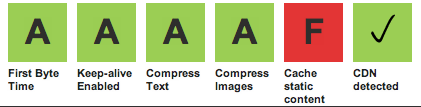
\includegraphics[width=0.5\textwidth]{figuras/lado_cliente/google/page_results.png}
  \caption{Resultados obtenidos por www.google.com.uy}
    \label{fig.google_page_results}
\end{figure}

Este sitio obtiene el peor puntaje en la regla \emph{Cache static content} ya que cuatro de las imágenes que contiene el sitio y el favicon del mismo no contienen los encabezados
\emph{Expires} o \emph{Cache-Control: max-age}, lo cual implica que en cada visita que se haga a la página se enviará un pedido condicional por cada una para verificar si los
elementos no han sido modificados. En particular, el impacto que tiene esta regla en el caso de Google no es de mayor impacto, ya que los elementos que no cumplen con esta regla son pocos
y su tamaño es pequeño.

Por otro lado, cabe destacar que las pruebas realizadas también dependen del navegador dónde se realicen, ya que cuando se accede al sitio de Google con un navegador
distinto a Google Chrome o Mozilla Firefox, la página desplegará un logo del navegador Google Chrome para descargarlo, teniendo que realizarse un pedido HTTP extra.

\subsubsection{Wikipedia}

En la figura \ref{fig.wikipedia_page_results} se pueden apreciar los resultados obtenidos por el sitio \emph{www.wikipedia.org} según la herramienta \emph{web page test}. Este sitio
obtuvo puntaje perfecto en cuatro de las seis reglas \emph{Keep-alive enabled}, \emph{Compress text} y \emph{Compress Images}, \emph{First byte time} y el puntaje
más bajo en la regla \emph{Cache static content}. Por otro lado, este sitio no utiliza una \emph{CDN} (en la imagen esta regla aparece con una \emph{X}), lo cual reduce de
forma considerable su performance.

\begin{figure}[h]
\centering
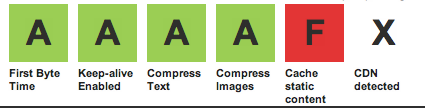
\includegraphics[width=0.5\textwidth]{figuras/lado_cliente/wikipedia/page_results.png}
  \caption{Resultados obtenidos por www.wikipedia.org}
    \label{fig.wikipedia_page_results}
\end{figure}

La herramienta \emph{Page Speed} le brinda un puntaje de setenta y dos sobre cien, y al igual que \emph{web page test} resalta el hecho de que trece de las imágenes (estáticas) que se encuentran en la página y el favicon de la misma no poseen los encabezados \emph{Expires} o \emph{Cache-Control: max-age}, por lo cual en cada visita a
la página se volverá a realizar un pedido para verificar si las imágenes continúan siendo válidas. Si se agregaran estos encabezados se ahorrarían catorce pedidos por visita al sitio, aumentando de forma considerable la performance del mismo.

Otra de las recomendaciones realizadas en este caso por \emph{Page Speed} es que varias de estas
imágenes pueden ser combinadas utilizando la técnica de \emph{CSS-Sprites}, reduciendo de esta forma los
pedidos por imágenes, incluso en la primer visita y con \emph{cache} vacío.

\subsubsection{Facebook}

Facebook obtiene un puntaje perfecto en todas las reglas verificadas por \emph{web page test} a excepción de una, \emph{Compress Images}, en la cual obtiene un 88\%. Esto se
debe a que las dos imágenes que aparecen en la página de inicio como propaganda pueden ser comprimidas para reducir su tamaño y de esta forma aumentar la performance del
sitio. En este caso las ganancias son prácticamente nulas, en el orden de 1.3KB. Los resultados de las distintas reglas según \emph{web page test}
se muestran a continuación.

\begin{figure}[h]
\centering
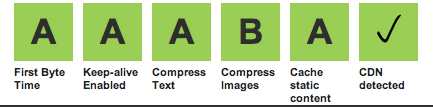
\includegraphics[width=0.5\textwidth]{figuras/lado_cliente/facebook/page_results.png}
  \caption{Resultados obtenidos por www.facebook.com}
    \label{fig.facebook_page_results}
\end{figure}

Otras de las recomendaciones hechas por esta herramienta es que se combinen las cuatro hojas de estilo provistas por facebook en un solo archivo, reduciendo de esta manera
la cantidad de pedidos realizados al sitio.

\emph{Page Speed} le otorga un puntaje de noventa y ocho puntos. Aunque las recomendaciones sean de baja prioridad, ayudan a mejorar la performance del sitio. Por un lado,
además de recomendar la compresión de las imágenes al igual que la herramienta anterior, también recomienda que se especifiquen el largo y ancho de las dos imágenes
que aparecen en la página inicial, para evitar de esta forma tener que calcular estos atributos cuando se esté renderizando la misma.

Por último recomienda utilizar \emph{Defer Parsing} para el siguiente javascript \emph{http://static.ak.fbcdn.net/rsrc.php/v2/y-/r/507fwwUzcWs.js} y para el que se encuentra
de manera \emph{inline} en el cuerpo del documento.

\subsubsection{Youtube}

Al analizar los resultados obtenidos por Youtube según la herramienta \emph{web page test}, se puede apreciar que los mismos no son muy distintos que los del resto de los sitios
previamente analizados. Los mismos se muestran a continuación.

\begin{figure}[h]
\centering
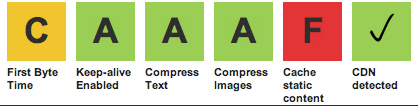
\includegraphics[width=0.5\textwidth]{figuras/lado_cliente/youtube/page_results.png}
  \caption{Resultados obtenidos por www.youtube.com}
    \label{fig.youtube_page_results}
\end{figure}

Uno de los principales problemas encontrados por esta herramienta es el \emph{First time byte}, el cual es aproximadamente trescientos milisegundos mayor al \emph{target time},
lo cual indica la posibilidad de generar mejoras del lado del servidor. Además, el sitio también falla en la regla \emph{Cache static content}, ya que once de los elementos presentes en la página no
contienen los encabezados \emph{Expires} o \emph{Cache-Control:max-age}, lo cual implica que se harán pedidos condicionales para analizar la validez de estos cada vez que se
realice una visita. Por otro lado, el sitio posee diecinueve elementos con un tiempo de expiración de seis horas y siete elementos con veinticuatro horas, esto se debe a que el
contenido del sitio es muy dinámico y cambia constantemente, en particular los videos destacados y recomendados.

Otra de las sugerencias realizadas por la herramienta es combinar las dos hojas de estilo en un solo archivo así como también los archivos con código Javascript, de esta forma
se ahorrarían dos pedidos HTTP en la primer visita el sitio.

Por otro lado, al evaluar el desempeño del sitio con \emph{Page speed} el mismo obtuvo un puntaje de ochenta y nueve sobre cien. Los principales motivos son la falta de fechas de
expiración en algunos componentes de la página, y el trato de las imágenes que realiza el sitio. 
El sitio contiene diez imágenes que son escaladas a un tamaño menor por el navegador y que si fueran provistas por el servidor con el tamaño correcto, permitirían un ahorro de 63.8KB.

Quince de las imágenes que componen el sitio no contienen los atributos \emph{height} y \emph{width} definidos, por lo cual el navegador puede tener que volver a posicionar elementos
del sitio una vez que las imágenes son descargadas.

\subsubsection{Yahoo}

Yahoo a diferencia de la mayoría de los sitios analizados con anterioridad, cumple con la regla \emph{Cache static content} de forma correcta, pero obtiene la peor calificación posible
en el cumplimiento de \emph{Compress Images}. Al igual que Youtube, este sitio no tiene un buen \emph{First time byte}, el mismo es cerca del doble que el \emph{target time},
aproximadamente 513ms. A continuación se muestran los resultados.

\begin{figure}[h]
\centering
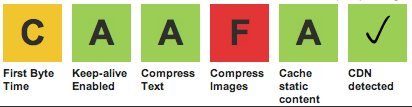
\includegraphics[width=0.5\textwidth]{figuras/lado_cliente/yahoo/page_results.png}
  \caption{Resultados obtenidos por www.yahoo.com}
    \label{fig.yahoo_page_results}
\end{figure}

El principal problema encontrado por esta herramienta son las imágenes que no se encuentran comprimidas. En particular, el sitio cuenta con diecisiete imágenes sin comprimir,
con las cuales se podrían ahorrar 218.4KB. Por otro lado, \emph{Page speed} recomienda englobar las veinticinco imágenes del menú lateral en un \emph{CSS Sprite}, de forma de
ahorrar veinticuatro pedidos la primera vez que se realiza una visita al sitio.
Otra de las recomendaciones hechas por estas herramientas es la combinación de dos archivos de código Javascript en uno solo para ahorrar de esta forma un pedido.

\subsubsection{Baidu}

Este sitio obtuvo uno de los puntajes más altos en relación al resto. \emph{Web page test} detecta dos fallas, la primera es que el favicon de la página no contiene
los encabezados \emph{Expires} o \emph{Cache-Control:max-age}. La segunda sugerencia consiste en el uso de una CDN para proveer los \emph{assets} estáticos. Debajo se encuentran
los resultados obtenidos por este sitio según \emph{Web page test}.

\begin{figure}[h]
\centering
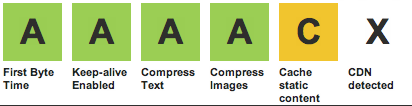
\includegraphics[width=0.5\textwidth]{figuras/lado_cliente/baidu/page_results.png}
  \caption{Resultados obtenidos por www.baidu.com}
    \label{fig.baidu_page_results}
\end{figure}

Por otro lado, \emph{Page speed} brinda sugerencias de baja prioridad. Sugiere utilizar la técnica de \emph{defer parsing}, ya que 40KB del código Javascript es parseado
durante la carga del sitio. Además, sugiere reducir el tamaño del logo principal para ahorrar de esta forma 386B, y especificar el tamaño de las dos imágenes que se
encuentran en el documento para que el navegador no tenga que reposicionar elementos una vez que se descargan estas imágenes.

\subsubsection{Live}

\emph{Web page test} otorga la peor calificación para este sitio al evaluar las reglas \emph{First Time Byte} y \emph{Cache static content}. En la figura \ref{fig.live_page_results}
se puede apreciar el puntaje obtenido por \emph{www.live.com} para todas las reglas.

\begin{figure}[h]
\centering
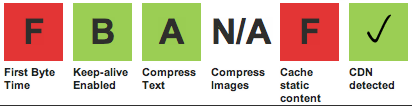
\includegraphics[width=0.5\textwidth]{figuras/lado_cliente/live/page_results.png}
  \caption{Resultados obtenidos por www.live.com}
    \label{fig.live_page_results}
\end{figure}

El motivo por el cual obtiene un puntaje tan bajo en la regla \emph{First Time Byte} es que el mismo tarda 2338ms en llegar, lo que implica que el tiempo de procesamiento
por parte del servidor es muy elevado. Por otro lado, la baja calificación obtenida en \emph{Cache static content} se debe a que una de las hojas de estilo, un archivo javascript
y cuatro imágenes no contienen los encabezados \emph{Expires} o \emph{Cache-Control:max-age}. Además, los javascripts y hojas de estilo correspondientes al login del sitio tienen una expiración de tan solo seis días y veinte horas.

Por otro lado, \emph{Page speed} encuentra varias sugerencias, una de prioridad media y el resto de prioridad baja. La sugerencia de prioridad media consiste en la compresión de
los elementos utilizando \emph{gzip} o \emph{deflate}, ya que una de las hojas de estilo y tres archivos javascript no se encuentran comprimidos, con lo cual se podrían ahorrar
29.6Kb.

Dentro de las sugerencias de menor prioridad, se encuentra la minificación de Javascript, hojas de estilo, el documento HTML y de un archivo .gif cuyo tamaño es mayor que un
paquete, por lo que reduciéndolo se puede reducir la latencia de ese pedido en particular.

Además, sugiere que el \emph{host} \emph{live.com} habilite el encabezado \emph{Keep-alive}, debido a que el mismo provee dos elementos, por lo que se podría
aprovechar la misma conexión para enviarlos y de esta forma ahorrar el \emph{overhead} de tener que establecer una nueva conexión TCP.

\subsubsection{QQ}

El sitio de noticias chino \emph{www.qq.com} no tuvo un buen desempeño en las pruebas realizadas por \emph{Web page test}. En la figura \ref{fig.qq_page_results} se pueden
ver los resultados obtenidos.

\begin{figure}[h]
\centering
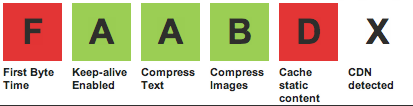
\includegraphics[width=0.5\textwidth]{figuras/lado_cliente/qq/page_results.png}
  \caption{Resultados obtenidos por www.qq.com}
    \label{fig.qq_page_results}
\end{figure}

Uno de los principales problemas de este sitio es el \emph{First time byte} ya que es cinco veces mayor al \emph{Target first byte time}, por lo que existe lugar para realizar
mejoras en el procesamiento del \emph{backend} para que la entrega del primer byte sea más veloz.

Otro de los problemas encontrados, al igual que en varios de los sitios analizados anteriormente, es una baja puntuación en la regla \emph{Cache static content}. Si bien el
sitio cuenta con ocho elementos que no contienen los encabezados \emph{Expires} o \emph{Cache-Control:max-age}, también cuenta con cuarenta y un elementos, de los cuales
cuatro tienen una fecha de expiración menor a cinco minutos, veintitrés elementos con fecha de expiración desde los diez minutos a una hora, doce elementos entre una y dos horas
y por ultimo dos elementos con tres días de expiración, todos plazos de validez demasiado pequeños según la definición de la regla.
Sin embargo, esto se debe a que se trata de un sitio de noticias, donde  las actualizaciones son constantes, por lo cual el puntaje obtenido en esta regla no es tan pertinente, ya que
los plazos cortos de expiración son por este motivo.

Otra de las recomendaciones hechas por esta herramienta es la compresión de las imágenes. Esto se debe a que el sitio cuenta con treinta y ocho imágenes que sin
comprimir o que están parcialmente comprimidas, lo cual permitiría ahorrar 89.9Kb de un total de 483.4Kb de imágenes.

\emph{Page speed} comparte algunas de las recomendaciones hechas por \emph{Web page test}, como la compresión de imágenes y la fecha de expiración de algunos componentes.
Si bien le otorga un puntaje de noventa y dos sobre cien, también sugiere minificar el HTML, el código Javascript y las hojas de estilo, pudiendo ahorrar de esta forma 7.3Kb.
Además, recomienda utilizar técnicas de \emph{Defer Parsing}, debido a que 104.1Kb de código Javascript es parseado durante la carga inicial del sitio y de esta forma se podría reducir el tiempo que tarda el navegador en cargar el sitio.

\subsubsection{Twitter}

Los resultados obtenidos por Twitter para las pruebas de \emph{Web page test} se muestran en la siguiente figura.

\begin{figure}[h]
\centering
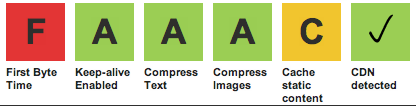
\includegraphics[width=0.5\textwidth]{figuras/lado_cliente/twitter/page_results.png}
  \caption{Resultados obtenidos por www.twitter.com}
    \label{fig.twitter_page_results}
\end{figure}

Se puede ver que el sitio desempeña bien en la mayoría de las reglas a excepción del \emph{First time byte} y \emph{Cache static content}. En el primer caso recibe una calificación \emph{F} a causa de que el valor del \emph{First time byte} es de 912ms cuando el \emph{Target first time byte} es de 414ms.

El sitio obtiene un puntaje medio en \emph{Cache static content} debido a que tres de los componentes tienen una fecha de expiración corta. En particular el
sitio mismo y el siguiente documento \emph{http://api.twitter.com/receiver.html} tienen una fecha de expiración de cinco minutos. Además, el Javascript de google-analytics
que es descargado tiene una fecha de expiración de doce horas.

Otra de las sugerencias realizadas por esta herramienta es la combinación de las dos hojas de estilo utilizadas por el sitio de forma de ahorrar un pedido HTTP. También se sugiere la
compresión de la imagen que es utilizada como fondo, ahorrando de esta forma 10.7Kb.

Por otro lado, \emph{Page speed} le otorga un puntaje de noventa y nueve sobre cien, brindando solo recomendaciones de baja prioridad. Entre ellas se encuentran la minificación
de Javascript y de HTML y la compresión de la imagen de fondo. También recomienda especificar las dimensiones de la misma para facilitar al navegador el proceso de renderizado
de la página.

\subsubsection{Amazon}
El sitio de Amazon obtiene un puntaje perfecto en la mayoría de las reglas verificadas por \emph{Web page test}. La calificación más baja que obtiene es \emph{B} en la regla
\emph{Cache static content}. Todos los resultados se muestran en la siguiente figura.

\begin{figure}[h]
\centering
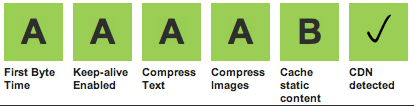
\includegraphics[width=0.5\textwidth]{figuras/lado_cliente/amazon/page_results.png}
  \caption{Resultados obtenidos por www.amazon.com}
    \label{fig.amazon_page_results}
\end{figure}

La razón por la cual obtiene esta calificación en \emph{Cache static content} es debido a que dieciocho componentes de este sitio no tienen los encabezados \emph{Expires}
o \emph{Cache-Control:max-age}. En este conjunto de componentes se encuentran el favicon de la página, un iframe, dos htmls, una imagen de propaganda, seis imágenes del sitio y ocho archivos de javascript. Las imágenes junto con el favicon deberían tener una fecha de expiración muy alta ya que las mismas son estáticas y no cambiarán en el futuro cercano.

Por otro lado, la herramienta recomienda combinar las tres hojas de estilo en una sóla para reducir de esta forma la cantidad de pedidos HTTP que se realizan al cargar la página.

Otra de las recomendaciones realizadas es la compresión de las imágenes ya que ocho de las imágenes contenidas en el sitio se encuentran parcialmente comprimidas o no poseen
compresión alguna, por lo que aplicando esta técnica se pueden ahorrar 44.4Kb, reduciendo el tiempo de descarga. También recomienda utilizar \emph{gzip}, debido a que dos
de los Javascript no se encuentran comprimidos y la mejora que se puede obtener es de 6.1KB.

Las últimas dos recomendaciones son mejorar el \emph{First time byte} que actualmente es de 250ms con un \emph{target first time byte} de 162ms, y utilizar \emph{CDN} para todos los contenidos estáticos, actualmente nueve componentes del sitio no son servidos por \emph{CDN}.

\emph{Page speed} comparte varias de las recomendaciones hechas por \emph{Web page test} y sugiere algunas más. En primer lugar sugiere la utilización de \emph{CSS Sprites}
para seis de las imágenes, incluyendo el logo de Amazon, fotos de iconos de distintas redes sociales y algunas imágenes utilizadas en el menú del sitio.
Por otro lado, sugiere reducir la cantidad de \emph{redirects}. Seis elementos realizan un \emph{redirect} antes de ser obtenidos.

Otra de las recomendaciones obtenidas es la minificación de las hojas de estilo, los Javascripts y el documento HTML, ya que de esta forma se pueden ahorrar aproximadamente 9Kb.
También recomienda especificar las dimensiones de las imágenes. Veinticinco imágenes presentes en el sitio no tienen especificadas sus dimensiones, lo cual puede implicar
que el navegador tenga que calcular el tamaño de algunos componentes y reposicionarlos a medida que renderiza el sitio.

\subsubsection{Otros sitios de alta concurrencia.}

Además de los sitios dentro de los diez más visitados, parece razonable analizar otros sitios de concurrencia alta. El objetivo de este pequeño análisis es mostrar que a pesar de que
algunos sitios sean muy concurridos y que tengan un respaldo económico importante, muchos no siguen las reglas de performance del lado cliente tan bien como podrían.
A modo de ejemplo se mencionan los siguientes sitios.

\begin{itemize}
	\item
	\textbf{\emph{NBA}} www.nba.com
	\item
	\textbf{\emph{The New York Times}} www.nytimes.com
	\item
	\textbf{\emph{CNN}} www.cnn.com
\end{itemize}

\subsubsection{NBA}
El sitio de la NBA marca un puntaje de setenta y dos puntos sobre cien, exactamente el mismo puntaje que el peor sitio de los diez más concurridos. Haciendo una mirada rápida a los
resultados, se puede ver que los errores más graves en cuanto a performance que comete el sitio no son difíciles de solucionar y tienen beneficios potenciales altos.

En primer lugar, el sitio no realiza \emph{caching} de manera correcta sobre las imágenes del menú, lo cual produce que en cada acceso al sitio el navegador deba volver a realizar
pedidos para obtener imágenes estáticas que seguramente no cambien en el corto y mediano plazo. Otro error grave relacionado con las imágenes mencionadas en el punto anterior
es que las mismas no están en un \emph{CSS Sprite} único, lo cual hubiera ahorrado al navegador una cantidad muy grande de pedidos, cumpliendo la regla de oro de la performance del lado cliente.

Una de las fallas más graves del sitio, no detectada en ningún otro sitio durante este análisis es el abuso de redirecciones. En el caso del sitio de la NBA, todos los pedidos de
recursos de avisos publicitarios se encuentran en rutas que terminan en redirecciones, no cumpliendo con una de las reglas de performance definidas por Souders. Otra sugerencia
brindada por la herramienta es habilitar algún tipo de compresión de los componentes, lo cual permitiría al sitio ahorrarse un total de 64\% del tamaño total de transferencia de los
recursos de tipo texto. Otro error bastante grave cometido por el sitio es la cantidad de código javascript que debe cargarse y ejecutarse antes de terminar de cargar la página.
Esto se podría mitigar utilizando algunas de las prácticas de \emph{defer parsing} propuestas por Souders.

\subsubsection{New York Times}

El sitio del diario New York Times marca un puntaje de setenta y ocho puntos sobre cien. Al igual que en el caso de la NBA, el sitio carece de ciertas optimizaciones de performance
que no necesariamente implican un esfuerzo importante para realizarse.

Revisando los resultados rápidamente se puede ver que el sitio tiene varias mejoras de performance pendientes relacionadas con las imágenes que contiene. Por un lado, varias
de las imágenes pueden ser comprimidas para reducir su tamaño. El tamaño de las imágenes de la página principal es más pequeño que el tamaño de las imágenes en el servidor, lo que deriva en que las imágenes que se transfieren sean de un tamaño superior al necesario desperdiciando ancho de banda. Si las
imágenes fueran del tamaño óptimo, el tamaño total de transferencia de las mismas se reduciría en un 53\%, aproximadamente 586.8KB.
Otra mejora posible referente a las imágenes es evitar el re escalado de imágenes por HTML.

Otra mejora sugerida por \emph{Page Speed} es aumentar el tiempo expiración en el cache de las imágenes del sitio. El problema en el caso del New York Times es que la página
principal se actualiza muchas veces al día, y las imágenes cambian en el correr del mismo. Dada la situación, parece innecesario especificar un tiempo de expiración largo para
imágenes que no se mantendrán en el sitio por demasiado tiempo. En cambio, se puede obtener una mejora al combinar las imágenes que pertenecen al menú del sitio en un
\emph{CSS sprite} único para reducir la cantidad de pedidos, este parece ser un error recurrente en la mayoría de los sitios analizados.

Viendo los resultados se pueden encontrar otras mejoras de menos impacto, como por ejemplo obtener recursos de URLs consistentes. Existen cuatro casos de imágenes idénticas
que se obtienen de rutas distintas, lo cual involucra realizar un pedido extra innecesario. Además la carga de javascript inicial es alta y podría reducirse por medio de técnicas de
\emph{Defer parsing} para no bloquear el renderizado del sitio.

Existen otras mejoras de menor impacto, como por ejemplo eliminar una redirección HTTP ahorrándose un pedido.
Otras mejoras posibles serían minificar el código javascript y HTML, aunque el espacio de mejora es bastante reducido.

\subsubsection{CNN}

El sitio de la CNN obtuvo un porcentaje de setenta y ocho puntos sobre cien en la prueba realizada con \emph{Page Speed}. Se pueden ver varias optimizaciones de performance
disponibles en común con los sitios de la NBA y el New York Times.

El problema más grave señalado por las pruebas es nuevamente con el \emph{caching} realizado por el sitio. En el caso de este sitio existen muchos recursos de tipos variados
que tienen un tiempo de expiración fijado en un número muy bajo. En el caso de las hojas de estilo y el código javascript, parecería razonable que se especificaran fechas de
expiración a largo plazo.

Sin embargo, en el caso de las imágenes el problema es un poco más complejo ya que al igual que el sitio del New York Times, las imágenes cambian según las
noticias que se muestren en portada. Las noticias se actualizan de forma regular cada quince minutos, por lo cual no sería razonable aumentar el tiempo de expiración a un valor muy
alto. 

Por otro lado, al igual que con los sitios de la NBA y del New York Times, las imágenes que conforman el menú del sitio son pedidas por el servidor por separado cuando podría
aplicarse la técnica de \emph{CSS sprites} para reducir la cantidad de pedidos.

El sitio de la CNN no tiene habilitada la compresión de elementos de tipo texto. Utilizando alguna técnica de compresión como gzip, se reduciría el tamaño de transferencia
total de estos elementos en un 78\%. El sitio de la CNN tampoco realiza ningún proceso de optimización de imágenes, lo cual podría reducir el tamaño total de transferencia de las
mismas en un 28\%. La cantidad de código javascript descargado cuando se accede a la página principal del sitio es elevado, por lo cual utilizar alguna técnica de \emph{Defer
parsing} podría reducir el tiempo en que el proceso de renderizado se detiene para ejecutar código javascript.

Al igual que en el caso de la NBA, existen cuatro rutas que terminan en redirección, realizando cuatro pedidos más de los necesarios, añadiendo RTTs extra y empeorando la
experiencia del usuario final.

\subsection{Caso de estudio en rails: Diaspora}

Dentro de los sitios más visitados construidos utilizando \emph{Ruby on Rails} se encuentra \emph{Diaspora} (www.joindiaspora.com). Dado que uno de los objetivos del proyecto de grado es identificar buenas
prácticas en aplicaciones de este tipo, se realizó una prueba utilizando \emph{Page Speed} y \emph{Web page test} sobre el sitio. El puntaje otorgado por ambas herramientas se encuentra por debajo del peor puntaje para los diez sitios estudiados anteriormente (Wikipedia).

Los resultados obtenidos por este sitio según \emph{Web page test} son los siguientes:

\begin{figure}[h]
\centering
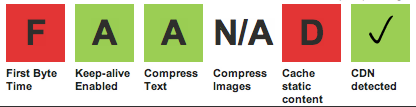
\includegraphics[width=0.5\textwidth]{figuras/lado_cliente/diaspora/page_results.png}
  \caption{Resultados obtenidos por www.joindiaspora.com}
    \label{fig.diaspora_page_results}
\end{figure}

Una de las principales fallas que encuentra \emph{Web test page} es el \emph{First Byte Time}, otorgándole un puntaje de 0 a este sitio. El \emph{target time} (tiempo
necesario para resolver las consultas de DNS, negociaciones de los sockets y SSL más cien milisegundos) para este sitio es de 225ms y el primer byte recibido por el navegador
desde el \emph{backend} tarda 1526ms en llegar. Esto implica que el procesamiento del lado del servidor es bastante lento y puede ser ampliamente mejorado.

El puntaje del sitio según \emph{Page Speed} es de cincuenta y siete sobre cien, a continuación se explican algunas de las causas. El sitio no cumple con ocho de las reglas definidas por la herramienta. Uno de los puntos que produce puntuación más baja es que los contenidos del mismo que están disponibles a través del servicio cloud front de amazon (los
archivos de javascript y CSS) no se comprimen (señalado por \emph{Page Speed} como un problema grave), lo que previene que el sitio reduzca el peso del total de los mismos en un
74\%, aproximadamente 496.6KB. En particular, \emph{Web page test} sugiere además la combinación de estos archivos en dos, uno que contenga el código
javascript y otro las reglas de CSS. En dicha categoría recibe un puntaje de cuarenta y cinco sobre cien.

El segundo punto más importante a mejorar según \emph{Page Speed} es la cantidad de código javascript que el navegador debe procesar. Para ser una página de inicio que solamente
consta de un formulario de ingreso típico del estilo usuario y contraseña, la cantidad de javacript es excesiva. El navegador debe detener el proceso de renderizado para procesar y
ejecutar el código javascript. En este caso parecería razonable utilizar técnicas de \emph{Defer Parsing}, pudiendo retrasar el procesamiento de los javascripts al cargar la página principal,
haciendo sentir al usuario que el sitio está disponible en menos tiempo.

Por otro lado, una de las mejoras más significativas sugerida por \emph{Web page test} es la utilización de los encabezados \emph{Expires} y \emph{Cache-Control:max-age}. En
particular, doce de los componentes de ésta página no contienen estos encabezados, algo considerado como una falla grave, teniendo en lo cuenta que varios de estos componentes son archivos con
código javascript y CSS que no cambia en el corto y mediano plazo, pudiendose ahorrar de esta forma varios pedidos HTTP en próximas visitas a la página.

\emph{Page Speed} también sugiere otras mejoras de menor impacto. Entre ellas se encuentra la omisión de utilizar la bandera \emph{keep-alive} (también sugerida por \emph{Web
page test}) del protocolo HTTP que permite que varios pedidos se realicen en una misma conexión TCP, ahorrando de esta forma el \emph{overhead} que tiene el inicio de una conexión TCP
y el \emph{slow start} de la misma.

Otro punto a mejorar, es la eliminación de código javascript dentro del cuerpo del documento HTML, lo cual produce que el navegador no pueda descargar de forma simultánea o
renderizar otros elementos.

